\section{Exercise 1c}
\lstinputlisting{Ex1c.py}
For this subquestion, we will try to make a fit again, but this time using a Poisson log-likelihood. In this we will be using the method without bins. The equation for this log-likelihood is: 

\begin{equation}
    -\ln{L} = \sum^{N_p-1}_{i = 0} \ln{[\mu(x_i|a,b,c)] + \int \mu(x_i|a,b,c) dx}, 
\end{equation}
where $\mu(x_i|a,b,c)$ is the model, with $x_i$ the data points. The integral is constant if we keep the model normalized. Therefore, we can remove that term for the minimization. Again, we will use a downhill simplex algorithm to find the minimum log likelihood, where we normalize every step. The results are shown below: 
\\
\\
\lstinputlisting{Ex1c.txt}


The results are shown in the Figure below.

\begin{figure}[h!]
  \centering
  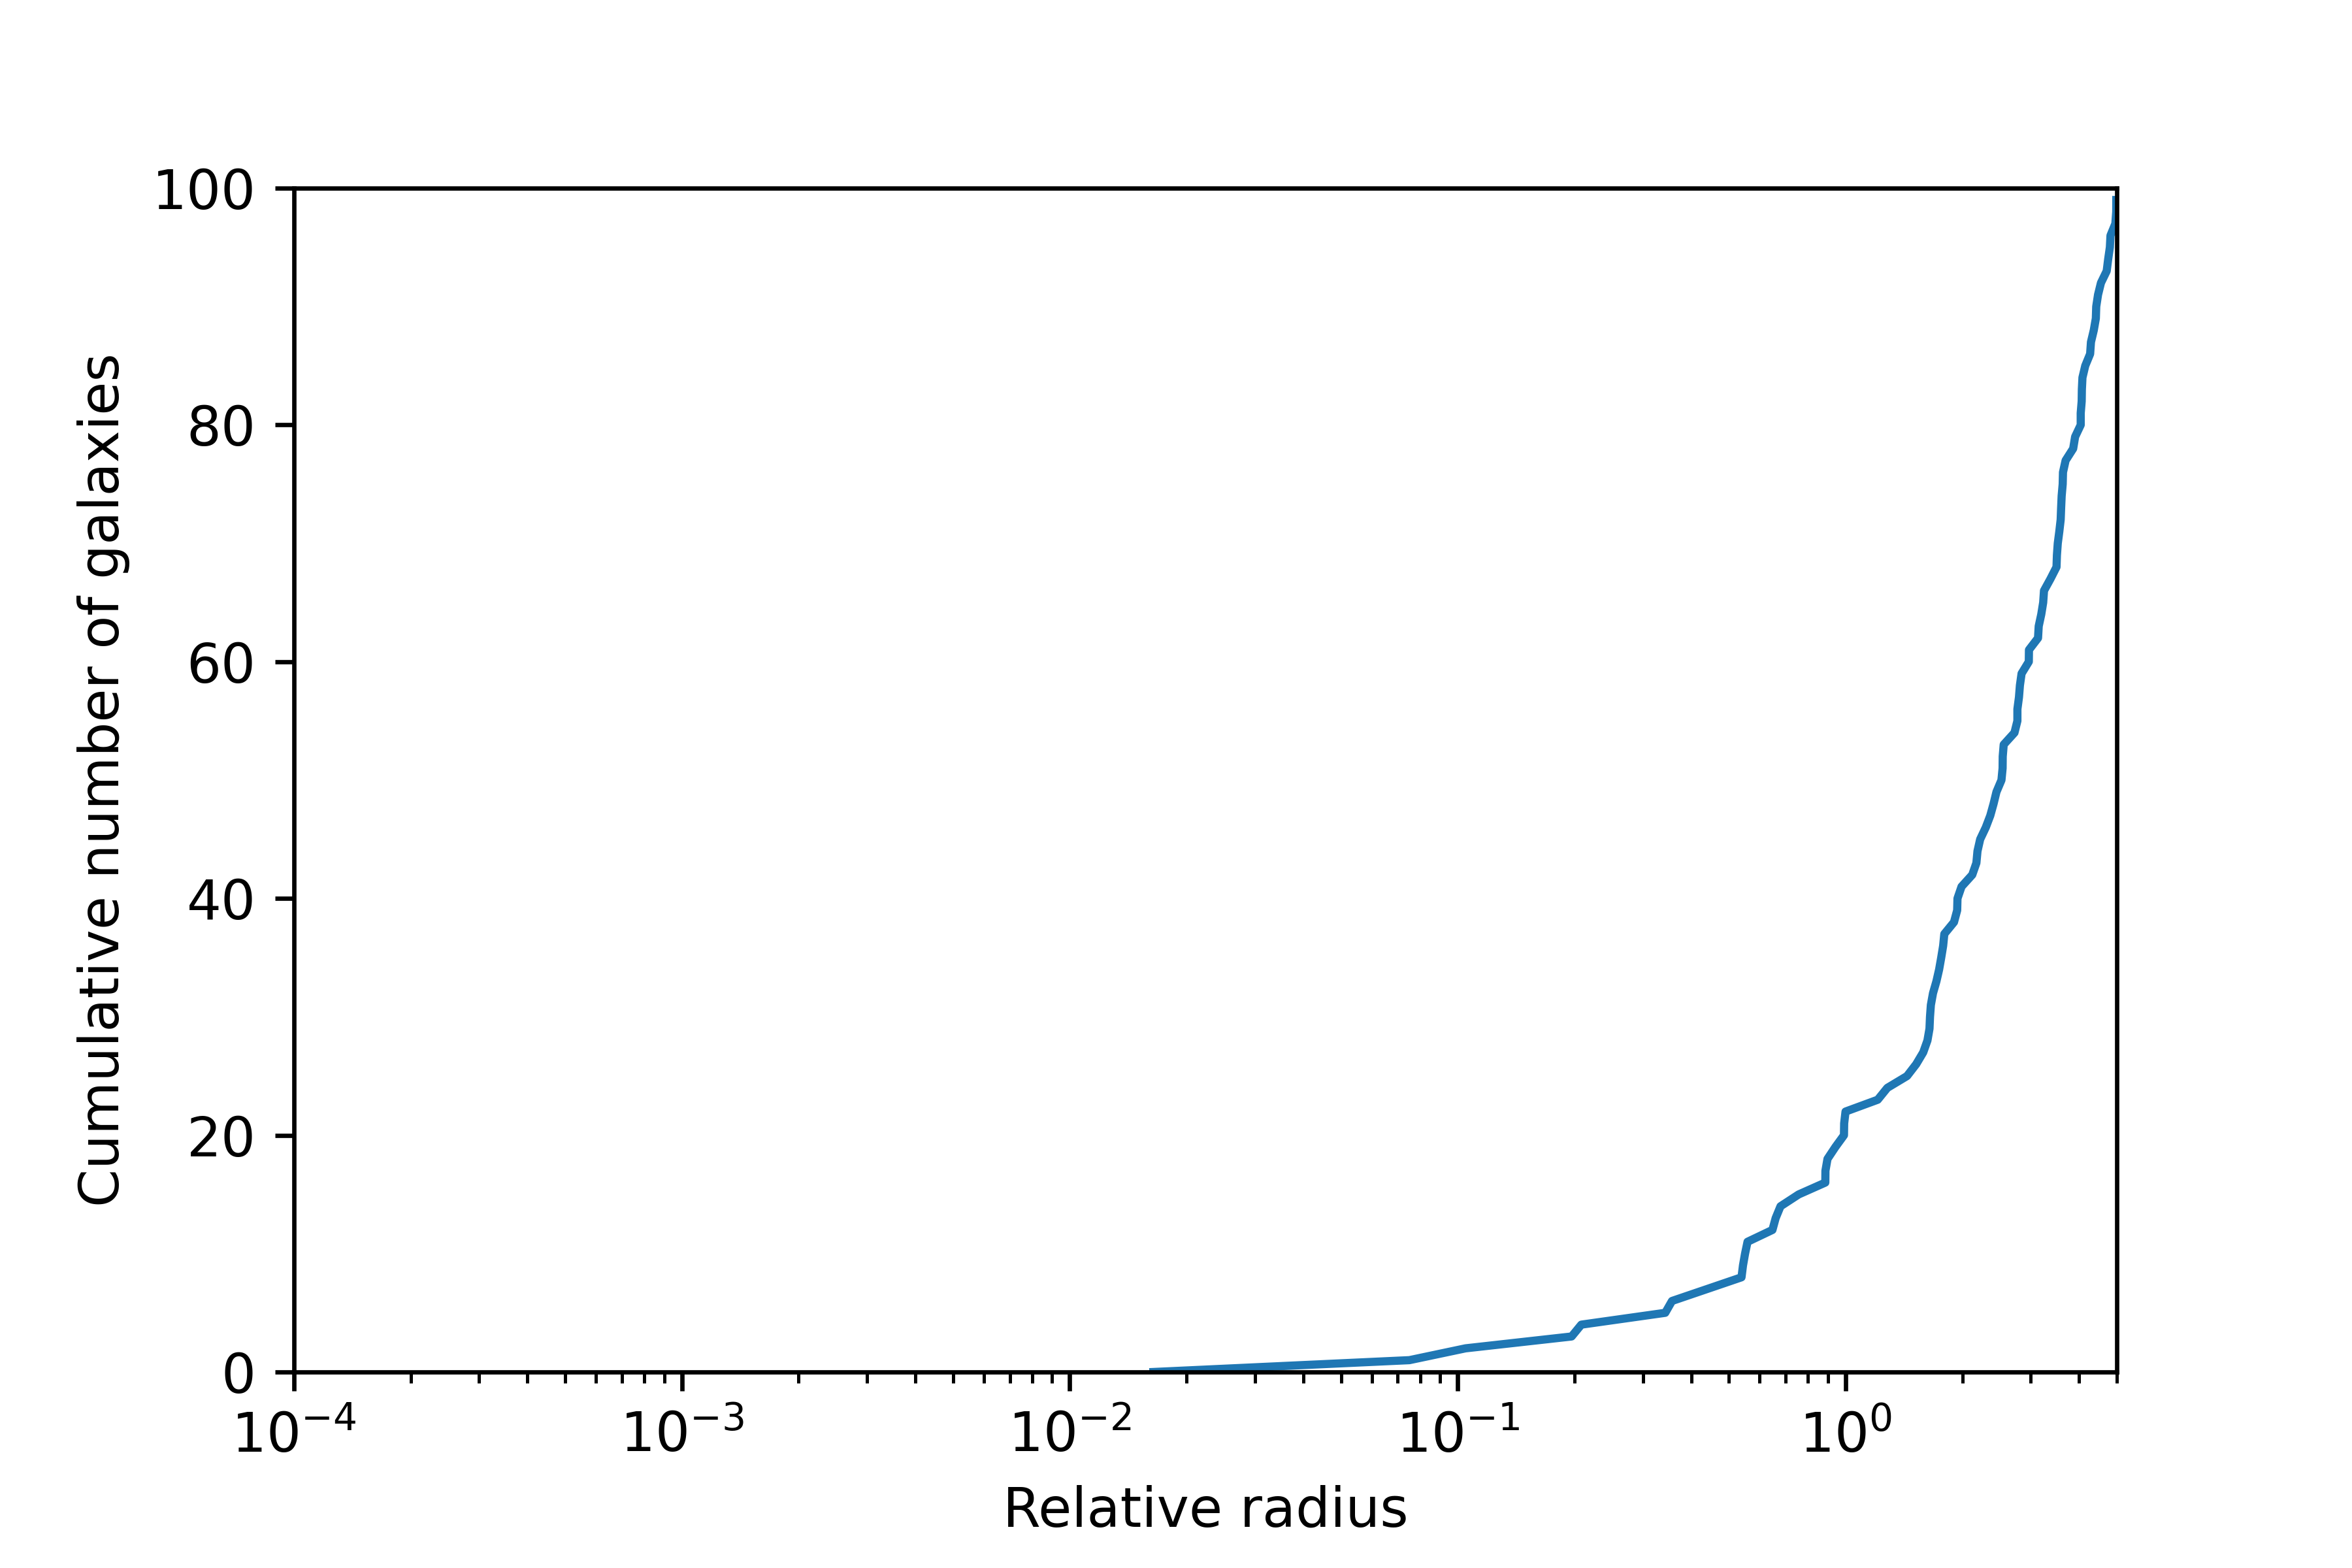
\includegraphics[width=0.9\linewidth]{my_solution_1c.png}
  \caption{A Poisson fit to the data. Again, we see a slight overestimation for some of the data sets. This could be due to the low amount of satellites with a low radius.}
\end{figure}
